\section{Introduction}
In this chapter we build on the empirical heat maps in Chapter 1. First, we develop a statistical model for spatial variation in hitter success probabilities. This involves generalized linear models (GLMs), some biomechanics, and polar coordinates. Second, we focus on heat map confidence intervals. We take a look at current best practices, and then provide an alternative.

\section{A Generalized Linear Model for Hitter Success Probabilities} % =========================

\subsection{Preliminaries}

We aim to create a statistical model to explain the variation of success probabilities through the hitting zone. Nonparametric methods, lacking contextually interpretable parameters, limit interpretability. We propose a parametric approach using biomechanically interpretable covariates. Existing research analyzes the biomechanics of the baseball swing \citep{Welch1995}, but no research links those results to spatial hitting results in a statistical model. To begin, we define preliminary indices and notation.

Let success indicator variable $Y_{ijklm}$ define a Bernoulli random variable with spatially varying mean \citep{Ross2002}. Let subscript $i = 1, \dots, n_{jklm}$ index hitter $j$ swings, in at bat $k$, against pitcher $l$, in year $m$. Let subscript $k = 1, \dots, n_{jlm}$ index hitter $j$ at bats against pitcher $l$, in year $m$. Let subscript $l = 1, \dots, n_{jm}$ index pitchers that hitter $j$ faced, with hitter-pitcher total $n_{jm}$; and let $m = 2007, \dots, 2016$ index year. Let $\pmb{s}_{ijkl} = (px_{ikl}, pz_{ijkl})\in \pmb{D} \subseteq \pmb{R}^{2}$ define the horizontal and vertical locations, respectively, of pitch $ijkl$ as it passes through the two dimensioned vertical face of the hitting zone\footnote{PITCHf/x\textsuperscript{\textregistered} records pitch locations in a three-dimensional coordinate system with horizontal x-axis, vertical z-axis, and y-axis running from the pitchers mound through home plate.}. The origin, $\pmb{s} = (0,0)$, lies at midpoint of the front edge of home plate, at ground level. From the umpire's point of view, pitches to the left of the origin correspond to negative values of $px$. Pitches that bounce before reaching home plate correspond to negative values of $pz$.  

In this study we make the simplifying assumption that location success probabilities depend on location and hitter only. Therefore, we dispense with subscripts $k, l,$ and $m$. We also assume, in this chapter, that swings occur---given hitter $j$ and pitch location $\pmb{s}_{ij}$---as statistically independent Bernoulli trials. Therefore, $Y_{ij}|\pmb{s}_{ij} \sim \text{Bernoulli}(p_{ij})$ where $\text{E}[Y_{i}|\pmb{s}_{ij}] = p_{ij}$. Accordingly, we revise and simplify the notation: let $i = 1, \dots, n_{j}$ index hitter $j$ swings, out of $n_{j}$ total recorded swings; and let vector $\pmb{X}_{ij}(\pmb{s}_{i})$ denote hitter $j$, location $\pmb{s}_{ij}$, swing $i$ covariates. A Bernoulli random variable suggests logistic regression, a GLM with logit link function, for relating covariate information to spatial success probability \citep{Myers2012}. The logit link, $logit(p) = log\left[p/(1-p)\right]$, maps $p$ with support $(0,1)$ to the positive real numbers. A GLM with logit link constitues a logistic regression equation, given by: 
\begin{equation}
\text{logit}(p_{ij}|\pmb{X}_{ij}(\pmb{s}_{ij})) = \pmb{X}_{ij}(\pmb{s}_{ij}) \pmb{\beta}_{j}.
\end{equation}
Vector of covariate coefficients $\pmb{\beta}_{j}$ contains parameters specific to hitter $j$. Next, we discuss and develop covariates.

\subsection{Rotational Biomechanics} % ==============

Why does Jhonny Peralta, and hitters in general, hit pitches in some locations better than others? We propose biomechanics underpin hitter location preferences. Notice that athletes, given the choice, carefully position their ball before swinging. Consider golf, a sport with a stationary ball, where the athlete chooses the exact athlete-to-ball distance, depth, and angle. 
  \begin{figure}[H]
	\centering	
	\includegraphics[scale=.45]{Images/Golf.jpg}
  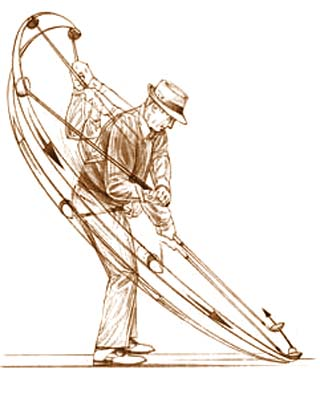
\includegraphics[scale=.6]{Images/Snead.jpg}
	\caption{Golfers position themselves with careful precision in relation to the ball, to achieve optimal impact. Deviations from this ideal lead to biomechanical adjustments and suboptimal results \citep{Cochran2005}.}
	\end{figure}
Indeed, golfers position themselves very precisely in relation to the ball to achieve optimal impact \citep{Cochran2005}. If the impact point deviates from the optimal location biomechanical adjustments hurt performance. Or consider tennis, similar to baseball in that a moving ball approaches, but different in that the player has freedom to position him/herself relative to the incoming ball. Once again, tennis players strive to hit the ball at a specific point in their stroke, a precise distance from the ground and from their body, with precise depth \citep{Elliott2006}. 
  \begin{figure}[H]
	\centering	
	\includegraphics[scale=.4]{Images/tennis2.jpeg}
	\caption{Tennis players strive to hit the incoming tennis ball at a precise height and distance from their torso. Deviations from this ideal height and distance lead to a series of biomechanical adjustments, and ultimately suboptimal results \citep{Elliott2006}.}
	\end{figure}
As with golf, if the point of impact deviates from from the optimal location, biomechanical adjustment ensue, and performance suffers. Tennis provides a strong example, because players have {\it some} control over the point of impact, and results demonstrate the consequence of varying points of impact. For example, even novice viewers observe that a player barely reaching a ball returns it, on average, with less velocity and precision than a ball he/her has time to set up for.  

In both golf and tennis the ideal player-to-ball positioning depends on, at the very least, anatomy, biomechanics, and equipment. We submit the same dynamics affect baseball hitting. However, in baseball the hitter reacts to unpredictable ball location, without time to reposition him/herself in response to the location and trajectory of the incoming pitch. For these reasons, we turn to hitter-to-ball distance and angle measurements for covariates. 

\subsection{Biomechanical Covariates}

Future research may incorporate physical characteristics specific to individual hitters. At this stage we focus on biomechanical information content captured in pitch locations. To produce biomechanical covariates, we convert (rectangular coordinate) pitch locations to polar coordinates with a translated origin. As illustrated in Figure 3.3, we shift the origin to the bat's approximate moment-of-intertia (MOI) for a league average 6'2" hitter \citep{Fleisig}. The MOI coincides approximately with the intersection of the bat line at the moment of contact and the hitter's axis of rotation \citep{Welch1995}.
  \begin{figure}[H]
	\centering
	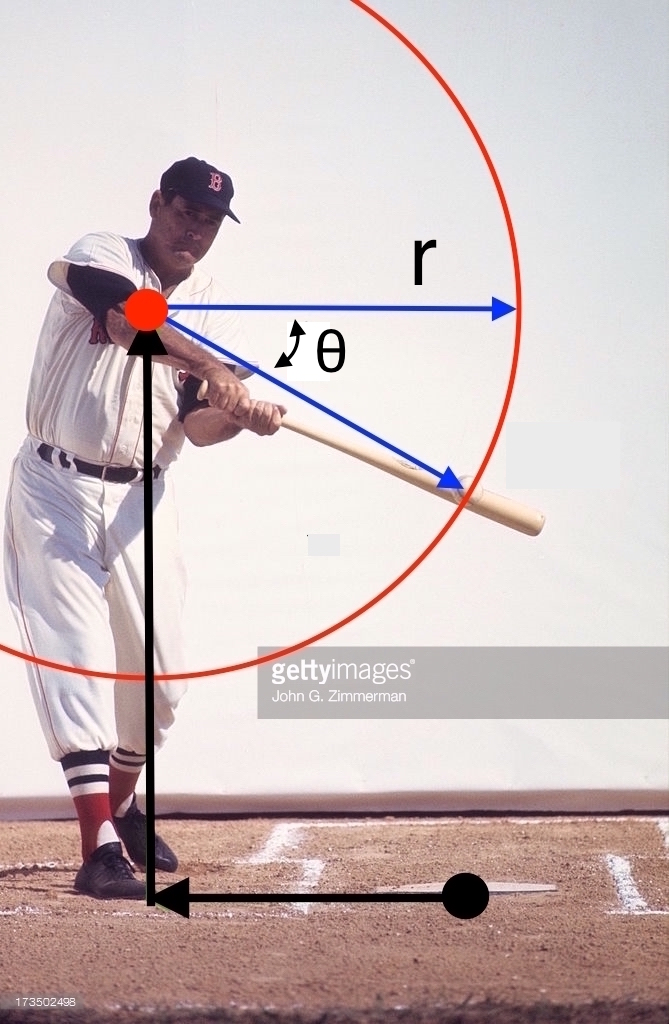
\includegraphics[scale=.16]{Images/WilliamsPolar.jpg}
	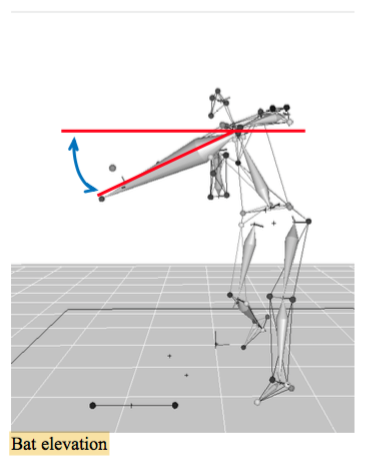
\includegraphics[scale=.07]{Images/Elevation.jpg}
	\caption{Ted Williams in ``The Science of Hitting,'' and baseball swing kinematic analysis at the American Sports Medical Institute \citep{Fortenbaugh2011}. We translate the origin (black dot) and rectangular coordinates to the new origin (red dot) in polar coordinates. We located the new origin at the bat's approximate moment of intertia (MOI) \citep{Fleisig}. Polar coordinates component $r$ gives the MOI-to-ball distance, and $\protect\theta$ gives the bat ``elevation.''}
	\end{figure}
Polar coordinate $r$ measures the distance, at contact, from the MOI to the ball. The kinematic analysis image on the right shows bat ``elevation,'' the angle below horizontal of the bat line, which serves as polar coordinate component $\theta$ \citep{Fortenbaugh2011}. 

As in golf and tennis, hitter-to-ball distances---too close to/far from the hitter, above/below the ideal point of impact---affect hitting performance. We use $r_{ij}$ and $\theta_{ij}$ terms for $\pmb{X}_{ij}(\pmb{s}_{ij})$ in equation 3.1.

\subsection{Generalized Linear Model} % =========================

Further biomechanical research extends beyond the scope of this study. Therefore, without biomechanical knowledge to inform us otherwise, we use $r$ and $\theta$ linear, quadratic, and interaction terms as covariates in our GLM linear predictor; $\pmb{X}_{ij}(\pmb{s}_{ij}) = \{r_{ij}, \theta_{ij}, r_{ij}\theta_{ij}, r_{ij}^{2}, \theta_{ij}^{2}, r_{ij}^{2}\theta_{ij}^{2}\}$. With $6 \times 1$ covariate vector $\pmb{X}_{ij}(\pmb{s}_{ij})$ in hand, we can define $\pmb{\beta}_{j}' =  \{\beta_{j0}, \beta_{j1}, \dots, \beta_{j6}\}$, and recall:

\begin{equation}
\text{logit}(p_{ij}|\pmb{X}_{ij}(\pmb{s}_{ij})) = \pmb{X}_{ij}(\pmb{s}_{ij}) \pmb{\beta}_{j}.
\end{equation}

% \begin{equation}
% \text{logit}(p_{ij}|\pmb{X}_{ij}(\pmb{s}_{ij})) = \beta_{j0} + \beta_{j1}r_{ij} + \beta_{j2} \theta_{ij} + \beta_{j3} r_{ij} \theta_{ij} +  \beta_{j4}r_{ij}^{2} + \beta_{j5} \theta_{ij}^{2} + \beta_{j6} r_{ij}^{2} \theta_{ij}^{2}
% \end{equation}

Note that given a hitter $j$, and pitch location $\pmb{s}_{ij}$, the elements of $\pmb{X}_{ij}$ are simply a trigonemtric function of $\pmb{s}_{ij}$ and the translated origin.

As a first step in exploring the effectiveness of the approach developed above, we fit the model to Johnny Peralta data (see Chapter 1). Let $j = P$, denoting player (P)eralta. We use Peralta's $n_{\text{P}} = 9177$ observed swings, and find maximum likelihood estimates of $\pmb{\beta}_{\text{P}}$ using an iteratively reweighted least squares algorithm (IRLS) \citep{Myers2012}. To delineate the estimation procedure, first recall the likelihood function for Bernoulli random variables,
\begin{equation}
\mathcal{L}(\beta|\pmb{y}) = \prod_{i=1}^{n} f(y_{i}) =  \prod_{i=1}^{n} p_{i}^{y_{i}}(1-p_{i})^{1-y_{i}},
\end{equation}
which gives log-likelihood, 
\begin{align}
\text{ln} \mathcal{L}(\beta|\pmb{y}) &= \sum_{i=1}^{n} \left[ y_{i} \text{ ln}\left(\frac{p_{i}}{1-p_{i}}\right) \right] + \sum_{i=1}^{n} \text{ ln }(1-p_{i}) \\
&= \pmb{\beta}'\pmb{X}'\pmb{y} - \sum_{i=1}^{n} \text{ln}[1 + \text{exp}(\pmb{x}_{i}'\pmb{\beta})].
\end{align}
To maximize the likelihood with respect to $\pmb{\beta}$, first take the derivative with respect to $\pmb{\beta}$,
\begin{align}
\frac{\partial \text{ ln} \mathcal{L}(\beta|\pmb{y})}{\partial \pmb{\beta}} &= \pmb{X}'\pmb{y} - \sum_{i=1}^{n}  \left[ \frac{1}{1 + \text{exp}(\pmb{x}_{i}'\pmb{\beta})} \right] \text{exp}  (\pmb{x}_{i}' \pmb{\beta}) \pmb{x}_{i} \\
&= \pmb{X}'\pmb{y} - \sum_{i=1}^{n} p_{i} \pmb{x}_{i} \\
&= \pmb{X}(\pmb{y} - \pmb{p}),
\end{align}
set it equal to zero,
\begin{equation}
\pmb{X}(\pmb{y} - \pmb{p}) = 0,
\end{equation}
and solve for $\pmb{\beta}$. The nonlinear relationship between $\pmb{p}$ and $\pmb{\beta}$ accounts for the challenge of solving the score equation above for $\pmb{\beta}$.
\begin{equation}
p_{i} = \frac{1}{1 + \text{exp}(-\pmb{x}_{i}'\pmb{\beta})}
\end{equation}
In such nonlinear systems, we turn to iterative methods in lieu of closed form solutions. Parameter estimation with IRLS depends on the correspondence between minimizing the least squares function and maximizing the likelihood, hence ``iteratively reweighted {\it least squares}.'' To see this, define weighted sum of squares
\begin{equation}
\text{S} = \sum_{i = 1}^{n}\left[ \frac{(y_{i} - p_{i})^{2}}{\sigma_{i}^{2}} \right]
\end{equation}



Figure 3.4 shows the Peralta empirical and fitted heat maps.
  \begin{figure}[!ht]
    \centering
    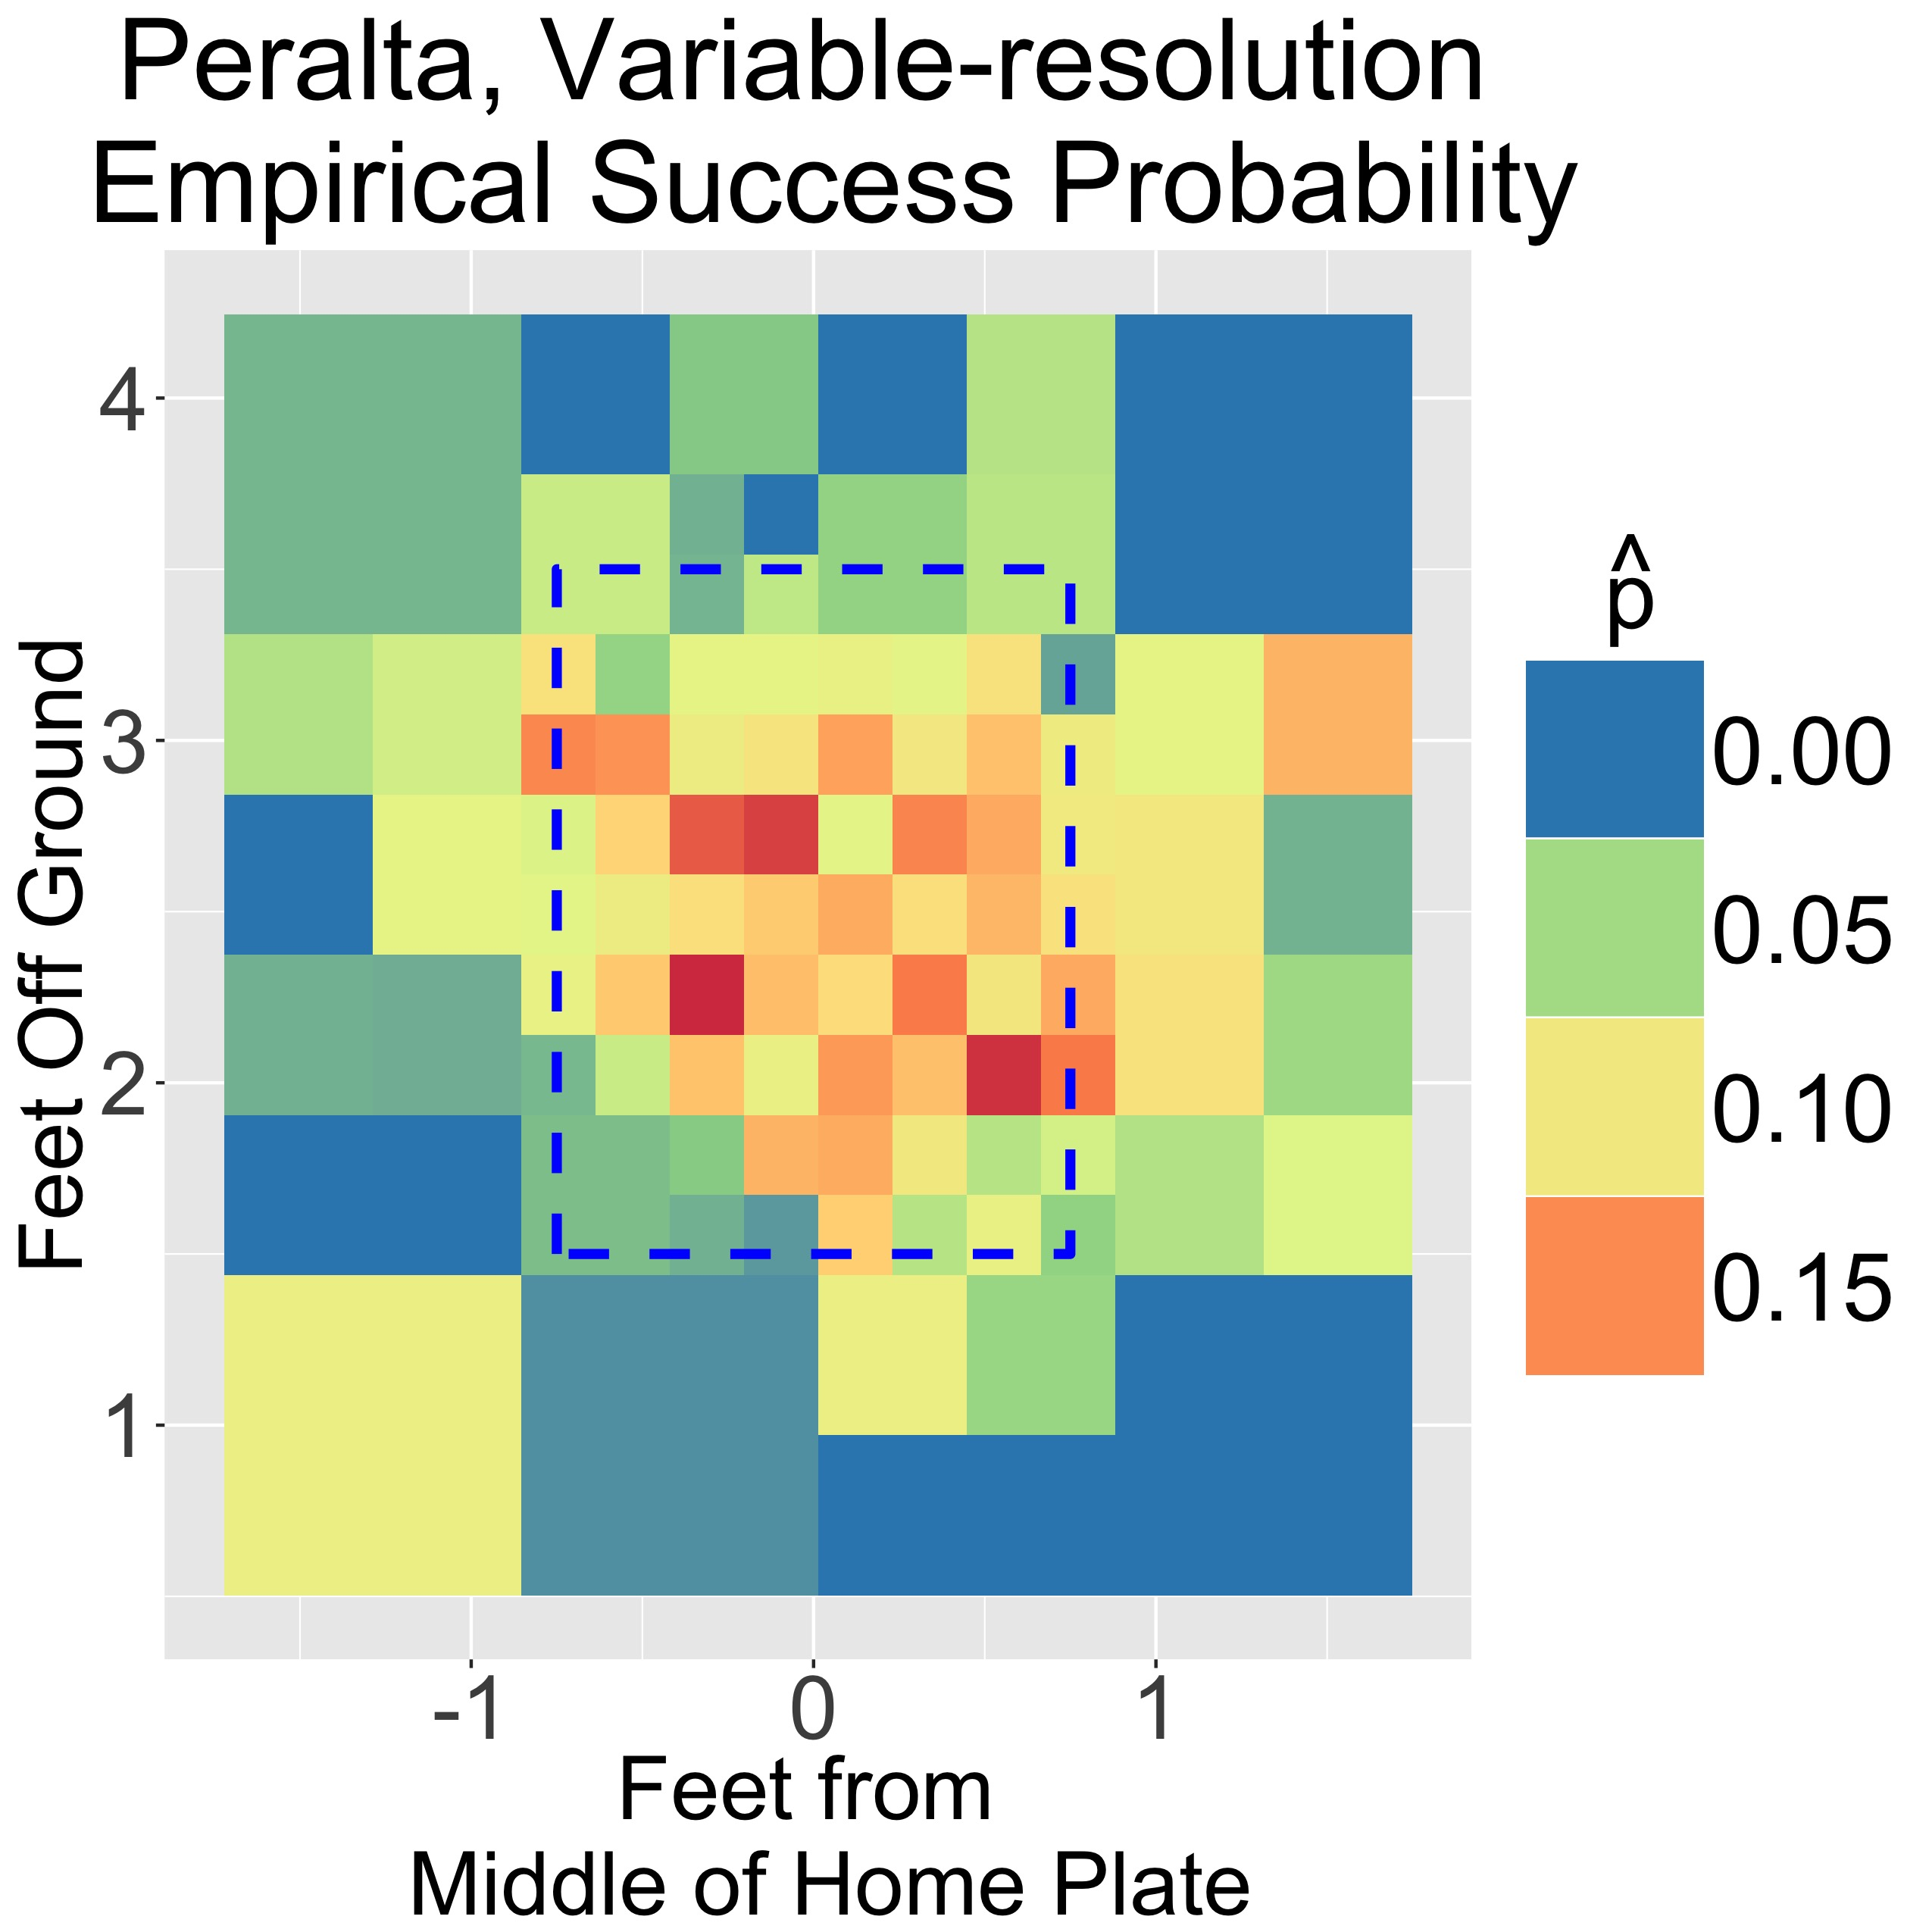
\includegraphics[scale=.08]{Images/Peralta_var-res.jpg}
    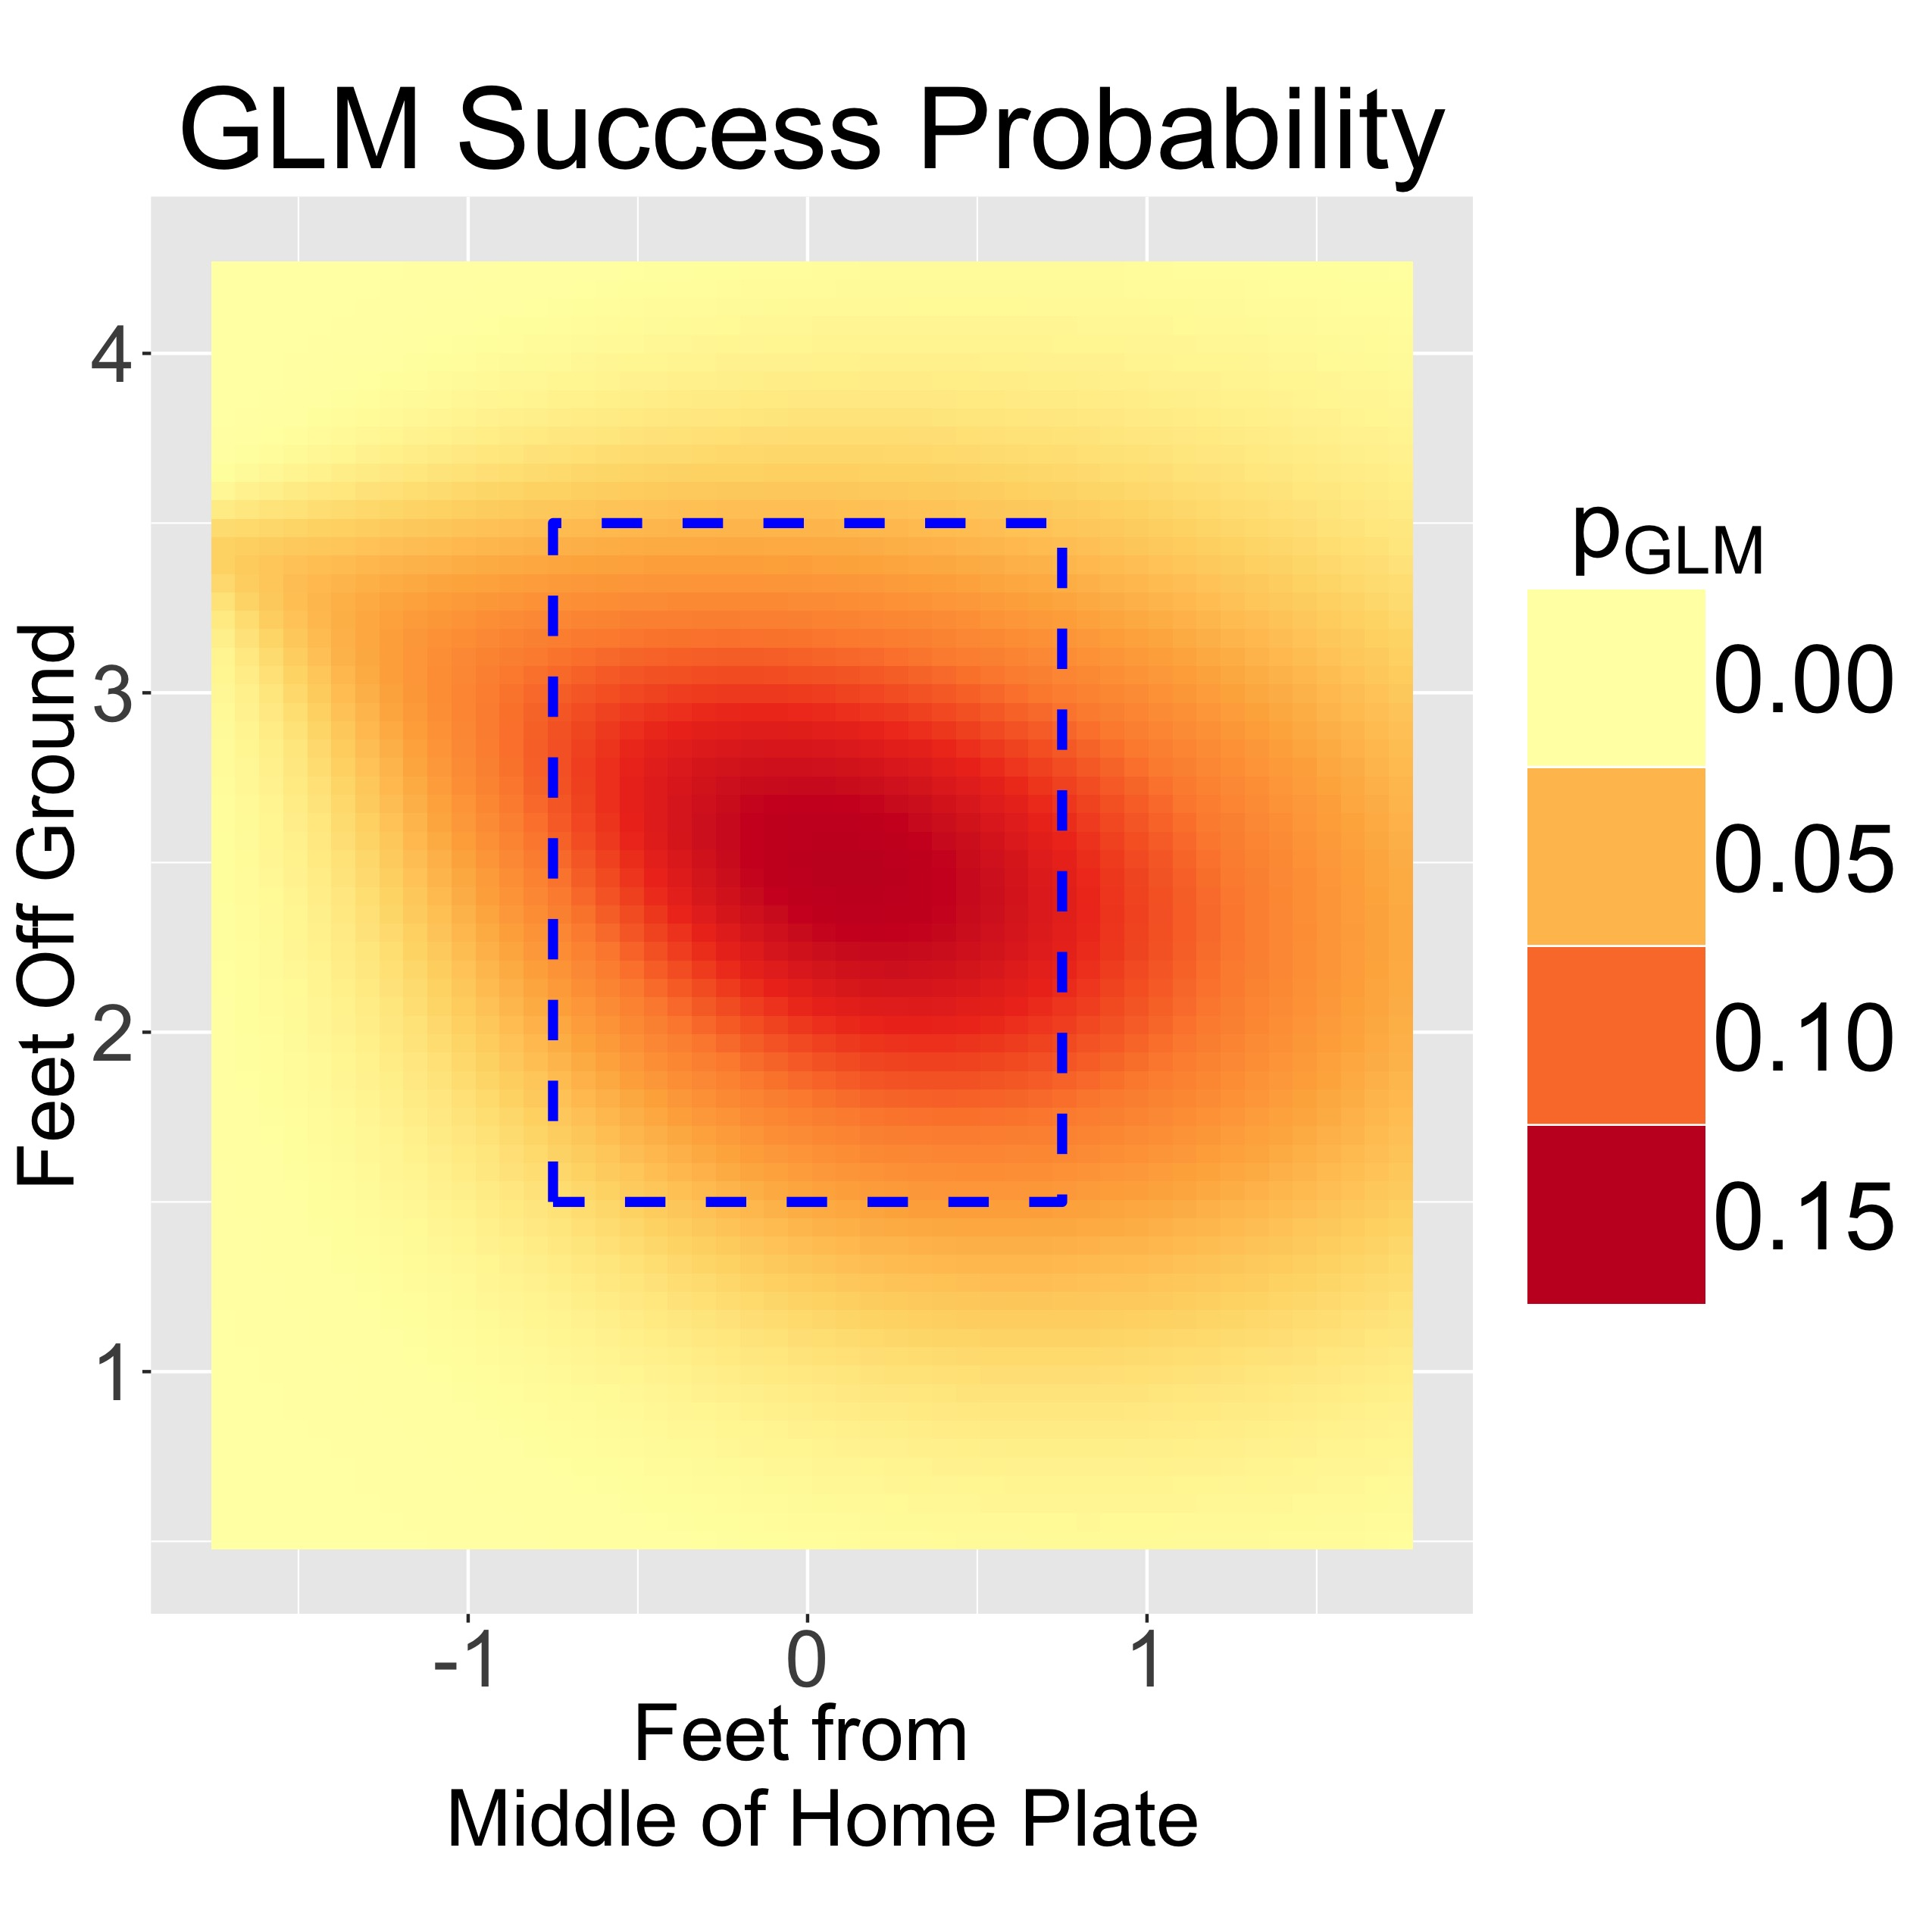
\includegraphics[scale=.08]{Images/Peralta_fit.jpg}
    \caption{Jhonny Peralta variable-resolution heat map and generalized linear model fit.}
  \end{figure}
The model {\it appears} well fit, but we turn to an established goodness of fit test for statistical validation.

\subsection{Hosmer-Lemeshow Goodness of Fit Test} % ================

The widely accepted Pearson $\chi^{2}$ test assesses goodness of fit for models with covariates that provide natural groupings \citep{Pagano2000}. Continuous covariate models, however, need an imposed grouping mechanism for a similar test. The Hostmer-Lemeshow test uses a grouping mechanism to imitate Pearson $\chi^{2}$ test structure, and tests logistic regression model goodness of fit \citep{Hosmer2013}. 

To construct the Hosmer-Lemeshow test, first define Bernoulli outcome vector $\pmb{y} = \{y_{1}, y_{2}, \dots, y_{n}\}^{\text{T}}$, and logistic regression model fitted probability vector $\hat{\pmb{y}} = \{\hat{p}_{1}, \hat{p}_{2}, \dots, \hat{p}_{n}\}^{\text{T}}$, where $E(y_{i}) = p_{i}$. Next, arrange fitted values $\hat{p}_{1}, \hat{p}_{2}, \dots, \hat{p}_{n}$ in ascending order, and divide them into $g$ evenly spaced percentile groups: $\frac{1}{g}, \frac{2}{g}, \dots \frac{g}{g}$. Therefore, $\text{Group 1} = \{\hat{p}_{i}|0 < \hat{p}_{i} < p_{1} \text{ where } \hat{\text{F}}(p_{1})=1/\text{g} \}$, for empirical CDF $\hat{\text{F}}(p)$. 

To define the Hosmer-Lemeshow goodness of fit test statistic, let $n_{k}$ be the number of observations in percentile group k. Then,
$$ \widehat{C} = \sum_{k=1}^{g} \left[ \frac{(\text{o}_{1k}-\hat{e}_{1k})^{2}}{\hat{e}_{1k}} + \frac{(\text{o}_{0k}-\hat{e}_{0k})^{2}}{\hat{e}_{0k}}  \right], $$
where
$$ \text{o}_{1k} =  \sum_{j=1}^{n_{k}}y_{j},$$
$$ \text{o}_{0k} =  \sum_{j=1}^{n_{k}}(1-y_{j}),$$
$$ \hat{e}_{1k} = \sum_{j=1}^{n_{k}}\hat{p}_{j}, \text{ and }$$
$$ \hat{e}_{0k} = \sum_{j=1}^{n_{k}}(1-\hat{p}_{j}).$$
Simplifying, 
$$ \widehat{C} = \sum_{k=1}^{g} \frac{(\text{o}_{1k}-n_{k}\bar{\hat{p}}_{k})^{2}}{n_{k}\bar{\hat{p}}_{k}(1-\bar{\hat{p}}_{k})},$$
where $\bar{\hat{p}}_{k}$ equals the group $k$ average predicted probability:
$$\bar{\hat{p}}_{k} = \frac{1}{n_{k}}\sum_{j=1}^{n_{k}}\hat{p}_{j}.$$
Notice $\widehat{C}$ matches the Pearson $\chi^{2}$ statistic under this grouping structure; and $\widehat{C}$ follows approximately a $\chi^{2}_{g-2}$, a chi-sq distribution with g-2 degrees of freedom \citep{Hosmer1980}, for the standard goodness-of-fit null and alternative hypothesis.
\begin{align}
H_{0}: & \text{ Model well fit.} \\
H_{1}: & \text{ Model not well fit.}
\end{align}
We use g = 10, follwing the \cite{Hosmer2013} recommendation based on their simulations \cite{Hosmer1980}. Our test statistic $\widehat{C} = 4.3758$, with eight degrees of freedom, gives a p-value of p = 0.8217. This strong failure to reject lends credibility to the biomechanical covariate approach. This validation suffices for now, and sets the stage for the most significant innovation in this chapter.

\section{Interactive Heat Map Confidence Intervals}

\subsection{Motivation}

A heat map presents a two dimensional surface of point estimates. Each (x,y) point on the surface maps a point estimate of a parameter to a color. As discussed in Chapter 2 with empirical heat maps, model fit heat maps also efficiently communicate the behavior of the parameter point estimates across the spatial domain. However, often the usefulness of a point estimate depends on confidence interval accompaniment, and therein lies the challenge: how to effectively present heat map confidence intervals (CIs)? This problem exists in numerous areas of application---in face, any field where heat maps are used. ``I've heard this question asked in other areas,'' remarked Dr Sarah Emerson \citep{Emerson}. Indeed, Dr. Emerson reports that in her own collaborative genomics research with Dr. Yanming Di, she and Dr. Di lacked a satisfactory heat map confidence interval option \citep{Emerson}, \citep{Emerson2012}. 

In the following two sections we present current heat map CI best practices, and then an alternative.

\subsection{Current Best Practices}

The currect heat map CI best practice consists of including two additional heat maps: the lower bound heat map and upper bound heat map. Sometimes the presentation includes maps for additional percentiles. For example, \cite{Cross2015} provide the following collection of heat maps to communicate prediction confidence.
  \begin{figure}[H]
	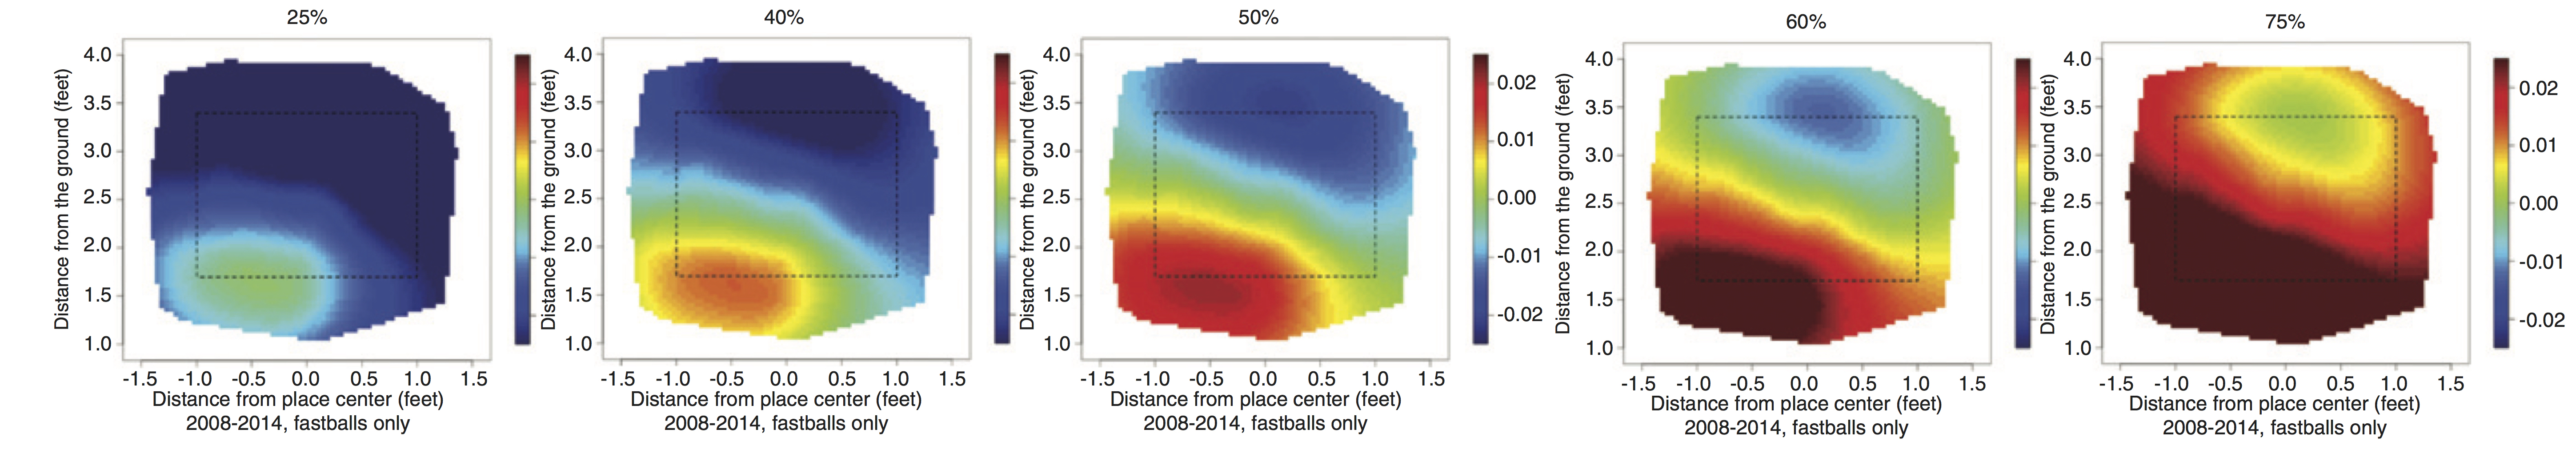
\includegraphics[scale=.07]{Images/CrossHMCI.jpg}
	\caption{In line with best practices, \cite{Cross2015} present four percentiles to convey confidence interval information for the point estimate heat map in the center. We submit this method resists easy, intuitive comprehension.}
	\end{figure}
This somewhat confusing heat map CI method seems conceptually and intuitively relatively inaccessible, especially compared to typical CI in two dimensions. For example, consider a hypothetical paremter and point estimate $\hat{\theta} = 2$, and hypothetical CI for $\hat{\theta}$ of (0,4). This combination makes plain its information content and structure; our familiarity with the number line contributes to easy comprehension.
  \begin{figure}[H]
  \centering
	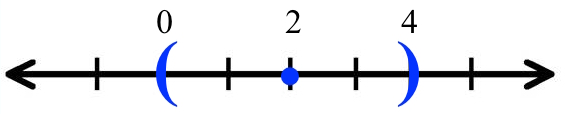
\includegraphics[scale=.6]{Images/NumberLine.jpg}
	\caption{Our brain readily understands and interprets the content of a confidence interval on the number line. On the other hand, our brain does not so easily understand and fill in missing intervals of the color spectrum.}
	\end{figure}
While one quickly, intuitively, and easily understands the content of the number line, we typically cannot so easily fill in missing segments of the color spectrum. With heat map CIs, {\it colors} represent the point estimate and confidence bounds. A point estimate of ``green'' with a CI of (purple, red) confounds.
  \begin{figure}[H]
  \centering
	
\includegraphics[scale=.75]{Images/Lower.jpeg}
	
\includegraphics[scale=.75]{Images/SpectrumPE.jpg}
	
\includegraphics[scale=.75]{Images/Upper.jpeg}
	\caption{This representation of a confidence interval on the color spectrum demonstrates the interpretive challenge. What stream of colors exist between each bound and the point estimate?}
	\end{figure}
However, we understand the CI more easily without missing spectrum segments, with the entire color CI visible as in Figure 6.
  \begin{figure}[H]
  \centering
	
\includegraphics[scale=.65]{Images/SpectrumCI.jpg}
	\caption{We understand a colored confidence interval without missing color segments, with the entire color CI visible. How do we achieve this for a heat map {\it surface}?}
	\end{figure}
This presentation improves comprehension immensely. But, how do we acheive this for a heat map {\it surface}? A continuous model maps innumerable point estimates on a surface, to a color; this makes a visible color spectrum CI for each point estimate infeasible. We propose a dynamic, interactive solution implemented with RStudio's Shiny \citep{Shiny}, \citep{RStudio}.

\subsection{Shiny Innovation}
The inimitable RStudio created the Shiny framework to facilitate interactive web application development. Deployed directly out of the RStudio integrated development environment (IDE) \citep{IDE}, Shiny applications provide a powerful new tool for presenting analytic results. We innovated a heat map CI method and implemented it with Shiny.

Recall the GLM model heat map for Jhony Peralta. Figure 7 shows the lower and upper 95\% pointwise CI heat maps.

  \begin{figure}[H]
	\centering
	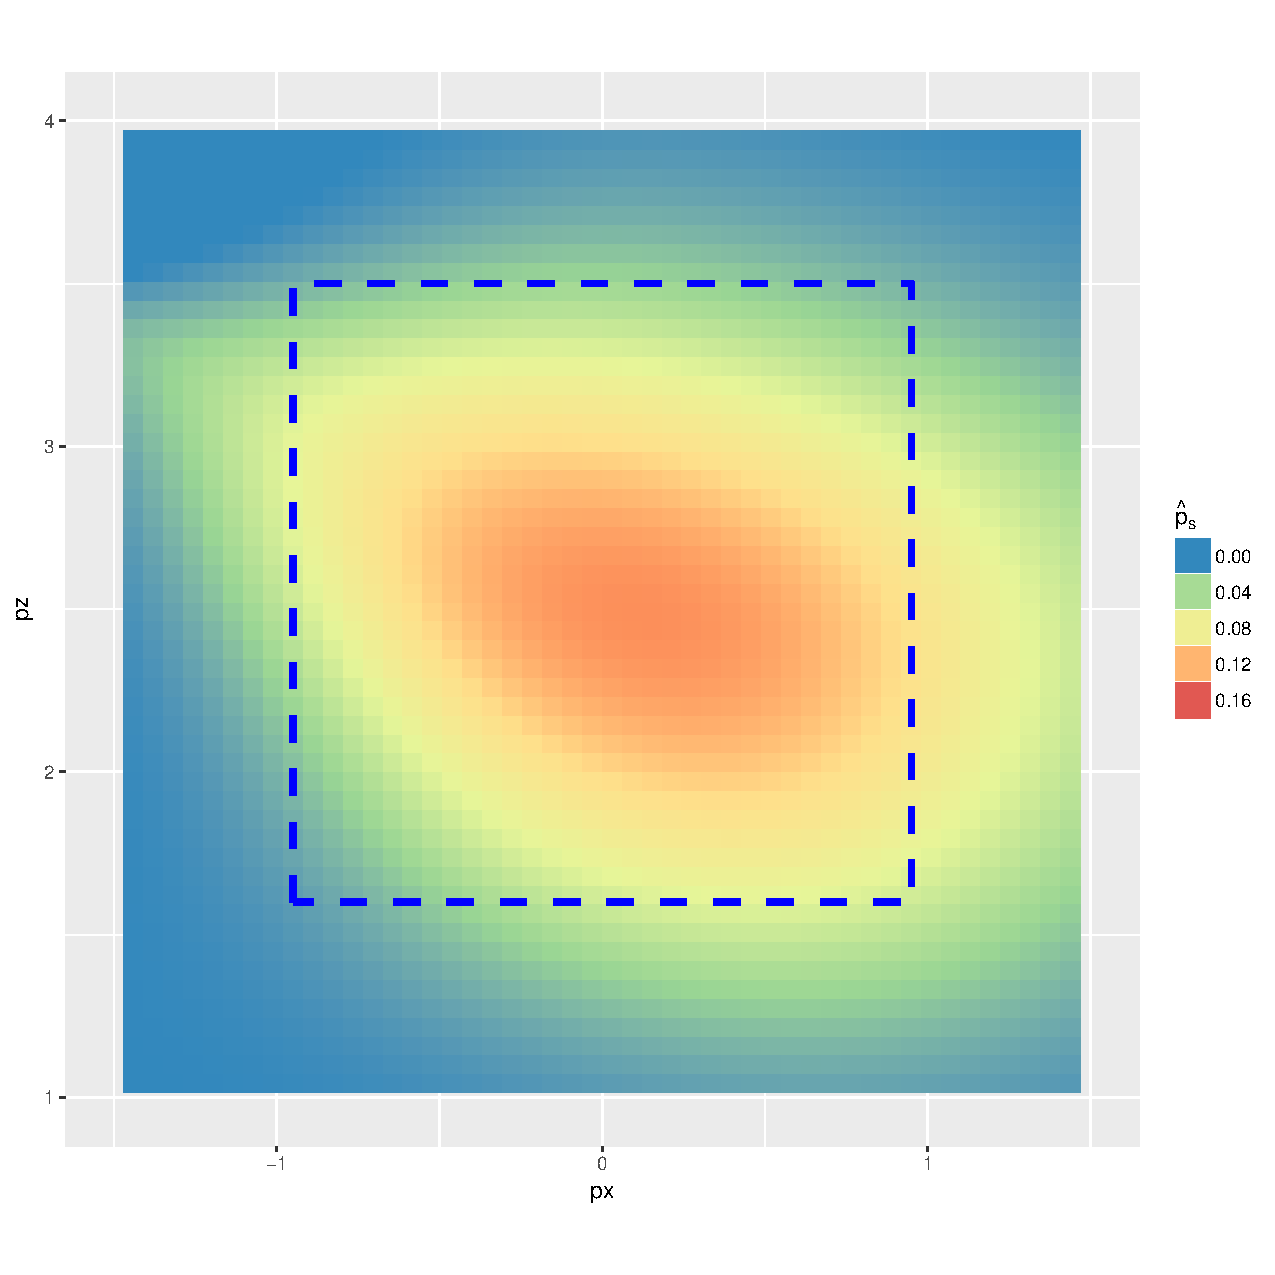
\includegraphics[scale=.2]{Images/Lower.pdf}
	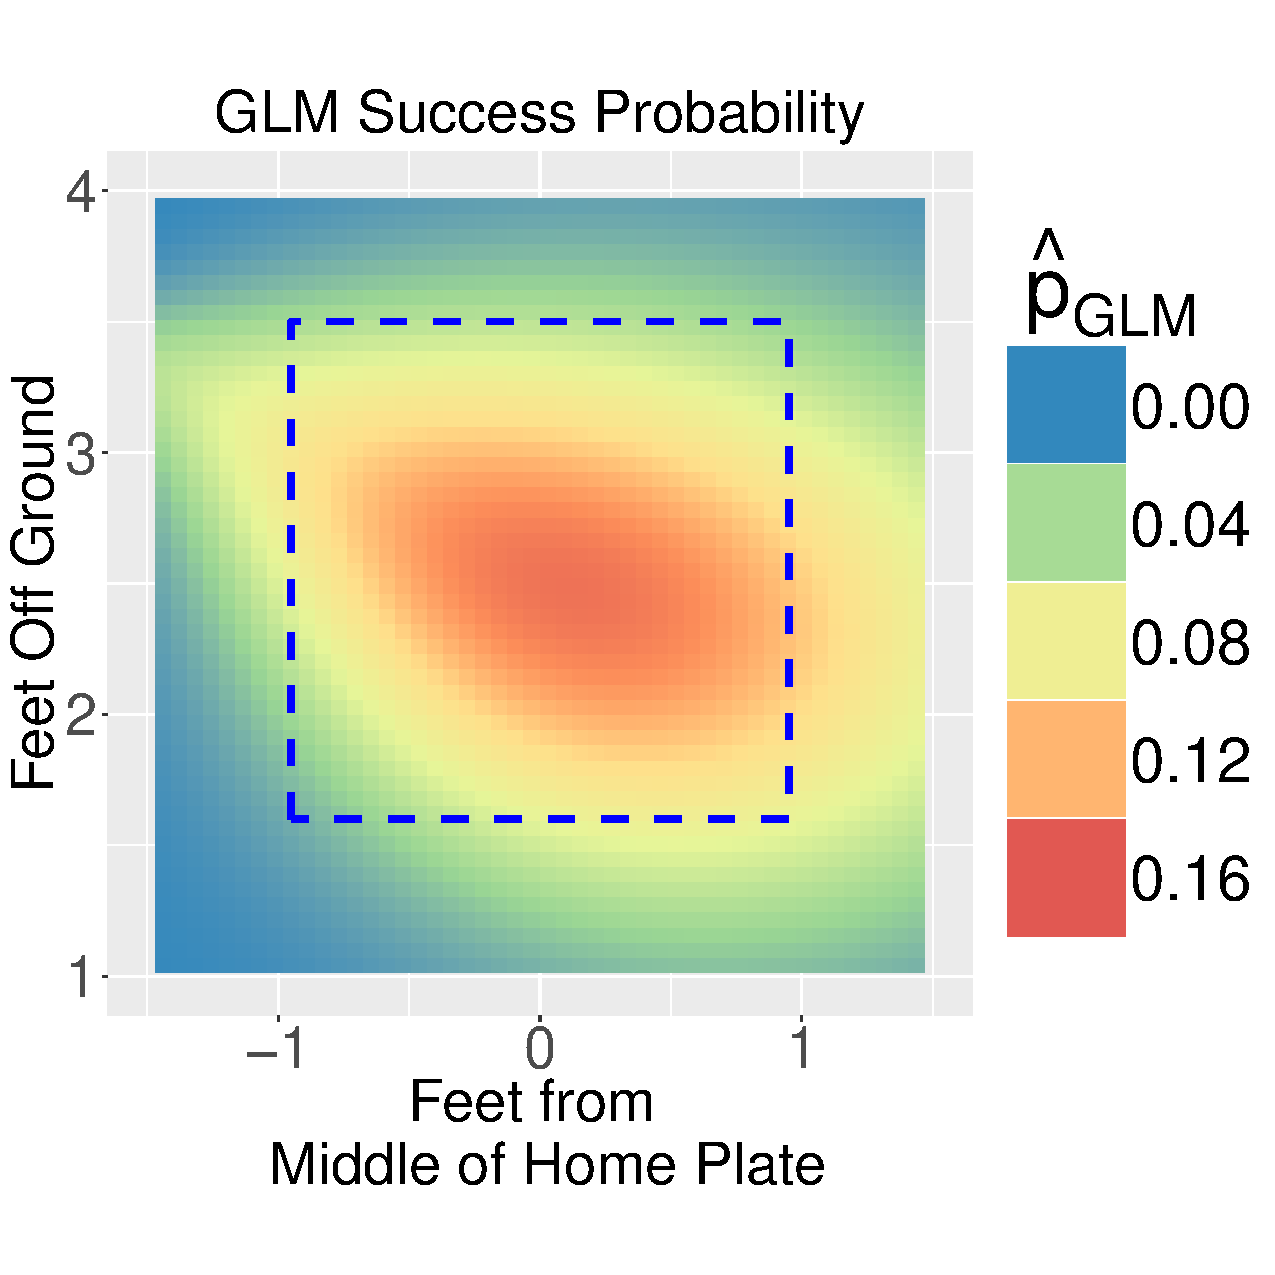
\includegraphics[scale=.25]{Images/Perralta_fit.pdf}
	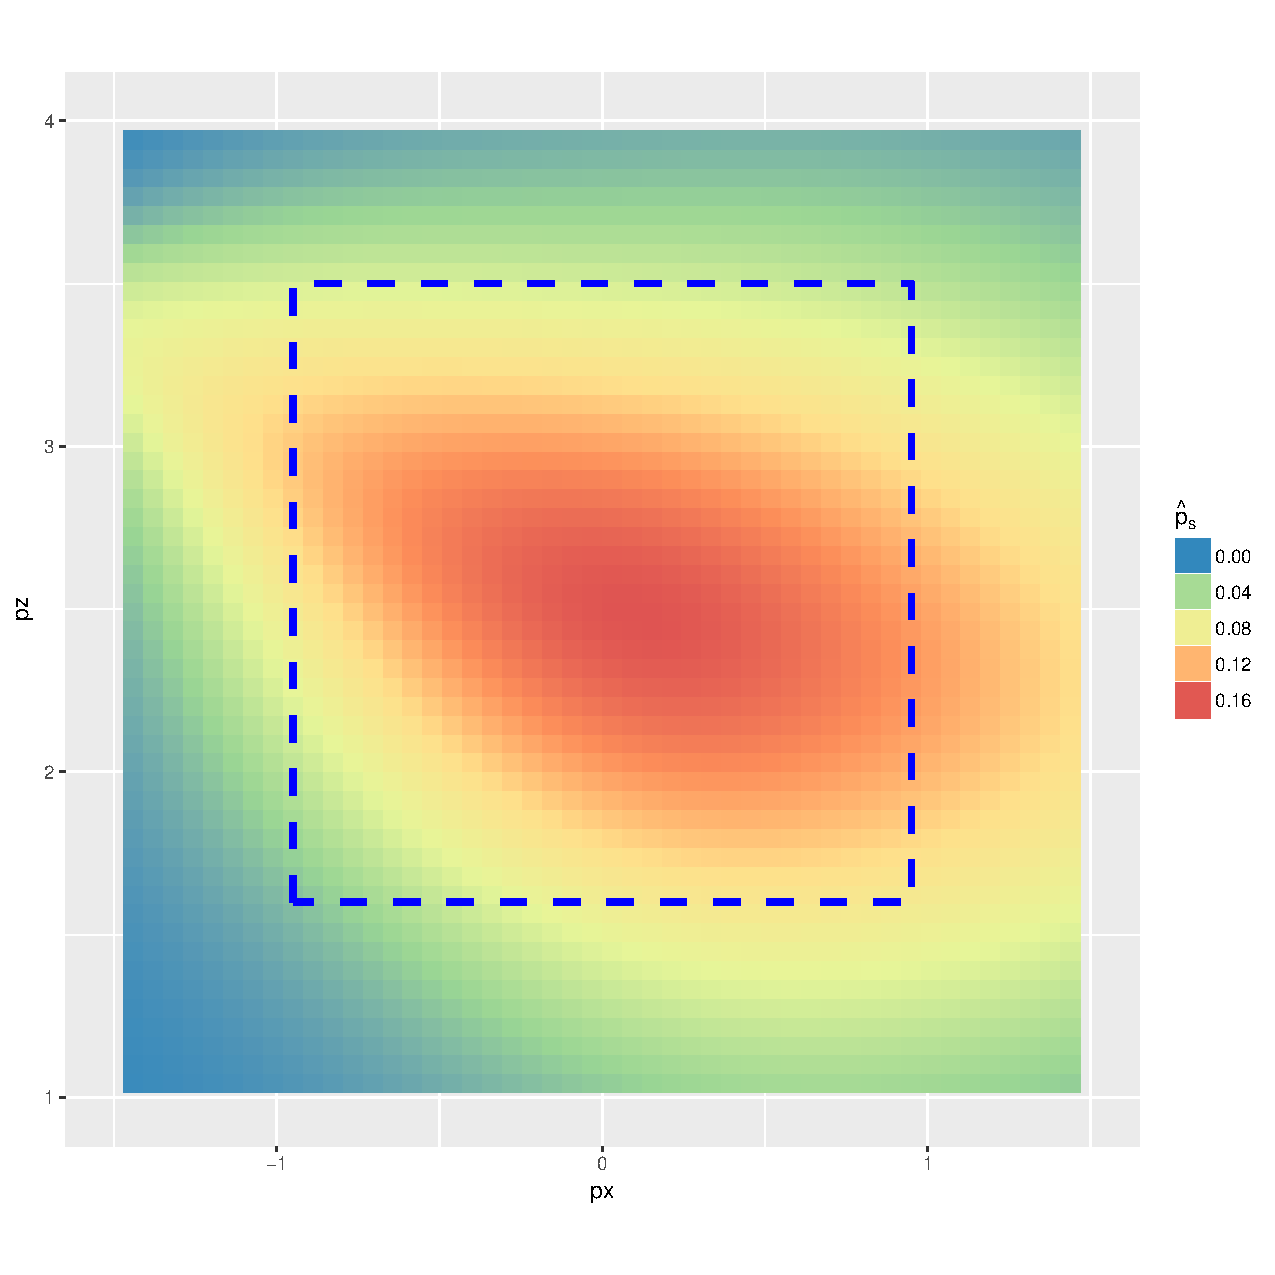
\includegraphics[scale=.2]{Images/Upper.pdf}
	\caption{Current best practices for a heat map confidence interval (CI). The generalized linear model fit for Jhony Peralta in the center, the pointwise CI lower/upper bounds on the left/right. Our interactive, dynamic heat map CIs improve interpretability.}
	\end{figure}
The heat map on the left gives the lower bound of the 95\% CI, the heat map in the middle gives the model fit point estimates, and the heat map on the right gives the upper bound of the 95\% CI. We removed labels from the left and right heat maps for simplicity. The challenge lies in filling the space, graphically and conceptually, between the bounds and point estimate. 

We fill the space by allowing the user, in real time, to interact with the Shiny slider that maps to the CI layers shown on-screen. \cite{Wickham2010} introduced a ``Layered Grammar of Graphics.'' A graphic maps a data attribute to an ``aesthetic.'' For example, in our heat map graphics we map the attribute $\hat{p}$ to the color aesthetic. In these terms, our interactive Shiny CI maps the slider a user interacts with to the CI layer visible on the screen. 

Figure 3.10 shows a static image of the interactive application. It includes a slider in the lower left. The user adjusts the slider to move {\it through} the CI.
  \begin{figure}[H]
	\centering
	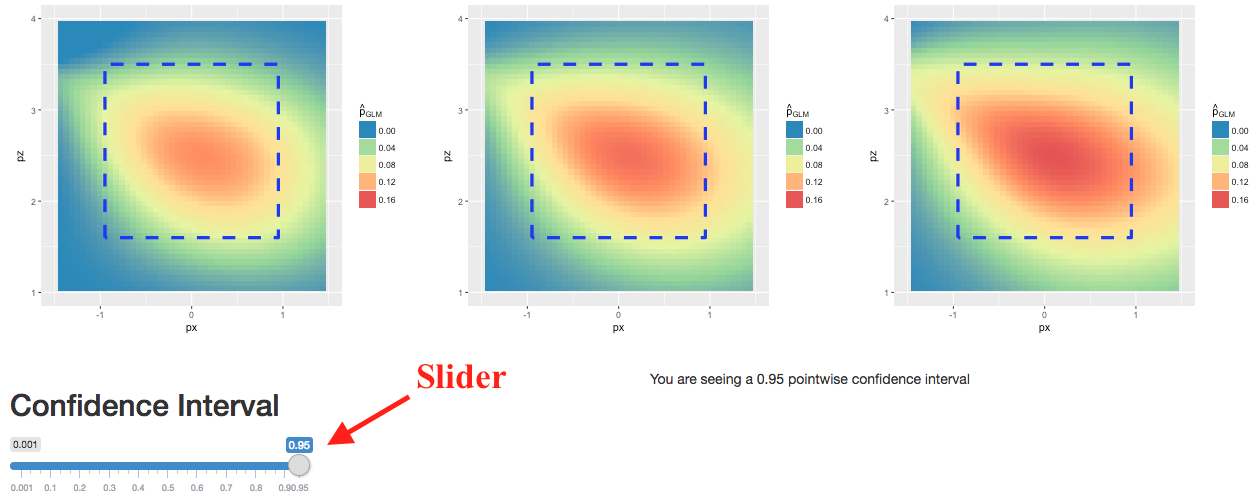
\includegraphics[scale=.35]{Images/95.png}
	\caption{We implemented our interactive heat map confidence intervals (CIs) with Shiny. The user adjusts the slider in the lower left to move {\it through} the CI. As the user adjusts the slider, the heat map bounds on the left and right give the appropriate layer.}
	\end{figure}
The slider specifies a CI level, which determines any particular CI width. As the user lowers the CI slider setting, the lower bound on the left and the upper bound on the right will ``move'' toward the point estimate, and look increasingly similar to the point estimate heat map in the middle. As the user increases the CI, the bounds ``move'' away from the point estimate: the lower bound colors cool, while the upper bound colors warm.

Figure 9 shows a sequence of static images in which the slider progressively narrows the CI.
  \begin{figure}[H]
	\centering
	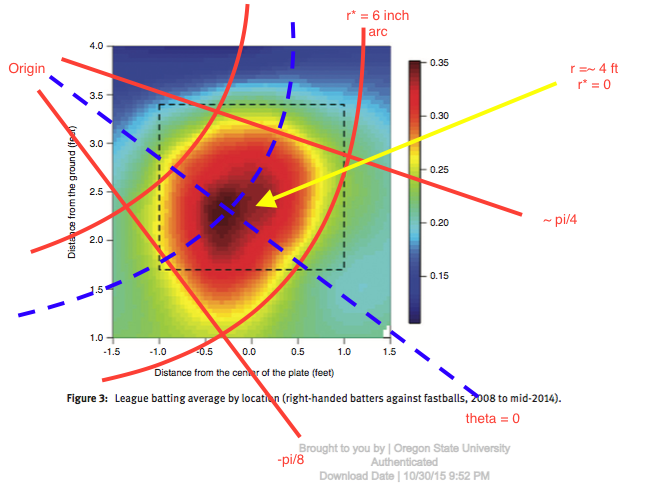
\includegraphics[scale=.25]{Images/1.png}
	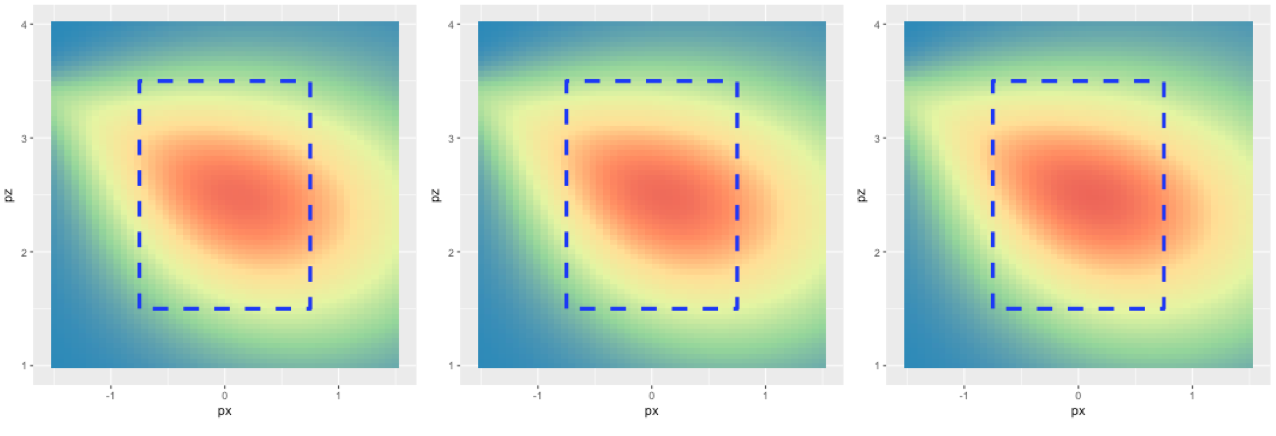
\includegraphics[scale=.25]{Images/25.png}
	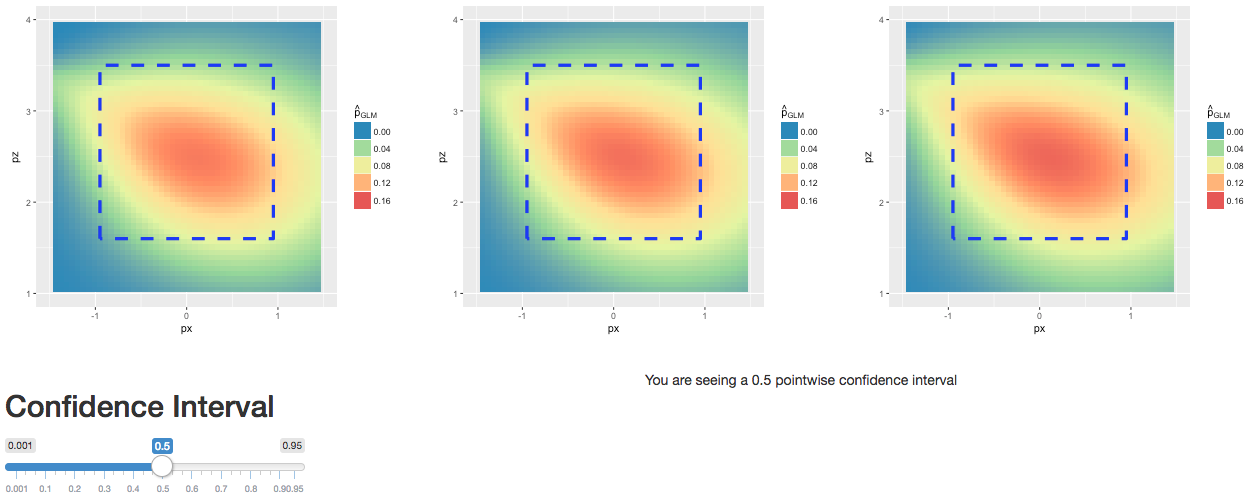
\includegraphics[scale=.25]{Images/50.png}
	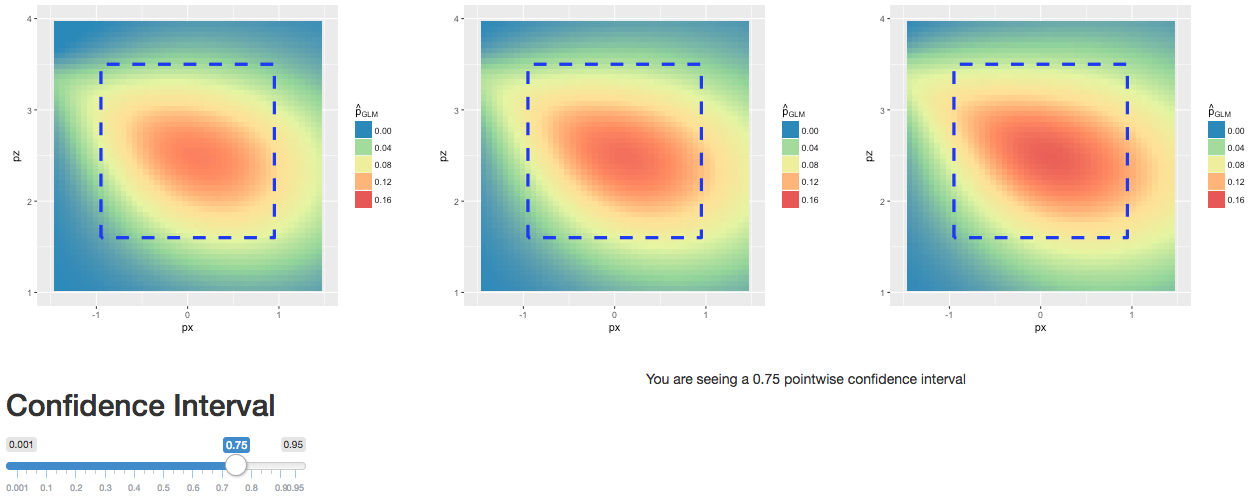
\includegraphics[scale=.25]{Images/75.png}
	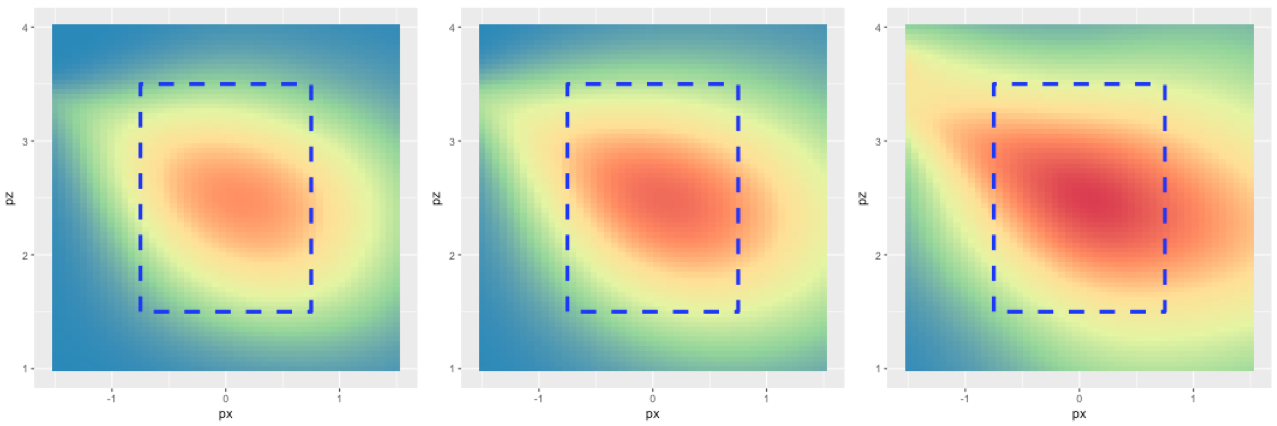
\includegraphics[scale=.25]{Images/99.png}
	\caption{An interactive confidence interval in Shiny lets the user move ``through'' the interval \citep{Shiny}. As the user adjusts the slider in the lower left (shown with first set of three maps), the heat map bounds respond accordingly. The interval gets increasingly wider moving down the rows: 1\%, 25\%, 50\%, 75\%, 99\%.}
	\end{figure}
Figure 3.11 shows the slider for the first row only. The top row shows a 1\% CI, followed by 25\%, 50\%, 75\%, and 99\% in the following rows. The first row contains three virtually identical maps, with the point estimate in the middle. Moving down the third (upper bound) column of maps, notice how the angled red egg shape subtly grows and elongates. This slow morphing culminates in the final image, where the red egg bleeds out of the strike zone to the upper left, and off the map to right. On the other hand, moving down the first (lower bound) column notice the red egg shrinking. The live, interactive application animates these effects, conveying them more vividly.

\subsection{Discussion}

While the paper version resembles the customary presentation, the actual interactive CI application comes to life as the user adjusts the slider. The user watches the CI bound maps morph into the point estimate map, which fills the intuitive gap explained above. Whereas our mind easily fills in a customary two-dimensional CI on the number line, this Shiny application now fills in the two-dimensional color surfaces of a heat map CI.

% \section{Chapter Appendix}
% 
% \begin{tabular}[b]{ l | c | c | c | r }
%     \hline
%     Covariate         & $\beta_{i}$ & MLE   & SE     &      p  \\ \hline \hline
%     N/A               & $\beta_{0}$ & -4.08 & 0.70 & $ <0.001$ \\ \hline
%     r                 & $\beta_{1}$ &  1.19 & 0.51 & $  0.018$ \\ \hline
%     $\theta$          & $\beta_{2}$ & -1.93 & 1.90 & $  0.311$ \\ \hline
%     $r*\theta$        & $\beta_{3}$ & -1.64 & 0.70 & $  0.064$ \\ \hline
%     $r^{2}$           & $\beta_{4}$ & -0.32 & 0.09 & $ <0.001$ \\ \hline
%     $\theta^{2}$      & $\beta_{5}$ & -3.92 & 1.10 & $ <0.001$ \\ \hline
%     $r^{2}*\theta^{2}$& $\beta_{6}$ & -0.46 & 0.21 & $  0.025$ \\ \hline
%     \hline
% \end{tabular}
